\chapter{Desarrollo e Implementación}\label{cap:desarrollo}

\section{Implementación del núcleo funcional}

Esta segunda etapa del proyecto se centró en la transformación de los diseños y
esquemas previos en un producto de software funcional. El objetivo primordial
consistió en construir una base tecnológica sólida que cubriera el ciclo de vida
completo del usuario dentro de la aplicación: desde el proceso de autenticación
inicial hasta la gestión avanzada de sus barajas.

Para asegurar la calidad del software, la implementación se llevó a cabo de forma
incremental y modular. Este enfoque, basado en el cumplimiento de hitos concretos y el
uso de commits atómicos, permitió validar de manera constante cada funcionalidad antes
de proceder a la siguiente, minimizando el riesgo de errores estructurales.

\section{Implementación del backend}

En el entorno de backend, se estructuró una API bajo el entorno de .NET 8 diseñada
para soportar operaciones sobre las barajas de usuarios autenticados.
Durante este proceso, se priorizó la separación de responsabilidades mediante el uso
de DTOs y validaciones independientes, lo que mejora la mantenibilidad del código y
evita el acoplamiento entre la lógica de negocio y la capa de transporte de datos.

Sobre esta arquitectura se consolidó el sistema CRUD completo para la entidad de
barajas: creación (CREATE), lectura (READ), actualización (UPDATE) y borrado (DELETE).
La lógica de actualización fue algo más compleja, ya que incluye la persistencia
dinámica de cartas dentro de cada mazo y la implementación de reglas de dominio
específicas, como el control de copias máximas permitidas y el tamaño total de la
baraja (60 cartas en total, con límites por nombre según juego).

Para garantizar la estabilidad de los datos externos se optimizó la comunicación con
los proveedores de cartas mediante el desarrollo de un mejor cliente HTTP. Se
realizaron ajustes pequeños en los algoritmos de búsqueda para asegurar que las
respuestas obtenidas desde fuentes como Pokémon o Magic fueran consistentes y
estuvieran listas para su procesamiento en el servidor.

Los extractos de código \ref{cod:dev-models-short},
\ref{cod:dev-controller-short} y \ref{cod:dev-validator-short} muestran,
respectivamente, un ejemplo de modelo, un endpoint de controlador y una validación de
reglas de baraja.

En el primer fragmento se observa cómo se modela una baraja en MongoDB con sus campos
clave: nombre, tipo de juego, lista de cartas y marca temporal de actualización.

\begin{lstlisting}[language={[Sharp]C}, caption={Fragmento de modelo Deck (C\#)}, label={cod:dev-models-short}, captionpos=b]
public sealed class Deck
{
    public string Name { get; set; } = string.Empty;
    public string GameType { get; set; } = DeckGameTypes.Pokemon;
    public List<DeckCard> Cards { get; set; } = new();
    public DateTime UpdatedAtUtc { get; set; } = DateTime.UtcNow;
}
\end{lstlisting}

El segundo fragmento resume el flujo básico del endpoint de creación: validar la
entrada, persistir en la colección y devolver la respuesta HTTP con el recurso creado.

\begin{lstlisting}[language={[Sharp]C}, caption={Fragmento de controlador para crear baraja (C\#)}, label={cod:dev-controller-short}, captionpos=b]
[HttpPost]
public async Task<IActionResult> CreateDeck([FromBody] CreateDeckRequest request)
{
    if (!DeckRequestValidator.TryValidateCreate(request, out var error))
        return BadRequest(new { message = error });

    await GetDecksCollection().InsertOneAsync(deck);
    return Created($"/api/decks/{deck.Id}", deck);
}
\end{lstlisting}

El tercer fragmento recoge dos de las reglas más relevantes del dominio: límite total
de cartas por baraja y número máximo de copias por nombre.

\begin{lstlisting}[language={[Sharp]C}, caption={Fragmento de validación de reglas de baraja (C\#)}, label={cod:dev-validator-short}, captionpos=b]
if (totalCards > MaxCardsPerDeck)
{
    errorMessage = $"Una baraja no puede superar {MaxCardsPerDeck} cartas.";
    return false;
}

if (copiesByName[normalizedName] > maxCopiesPerName)
{
    errorMessage = $"No puedes tener mas de {maxCopiesPerName} copias con el mismo nombre.";
    return false;
}
\end{lstlisting}

La API desarrollada sigue un diseño REST, estructurado en torno a recursos como
usuarios, barajas y cartas. Esta organización permite una separación clara de
responsabilidades y facilita la escalabilidad del sistema.

\subsection*{Documentación de la API}

Los endpoints implementados cubren tanto la autenticación como la gestión completa de
barajas, la colección de cartas del usuario y la comprobación del servicio.

\subsubsection*{Comprobación del servicio}

\begin{itemize}
	\item GET /: estado básico del backend.
	\item GET /api/health/mongo: comprobación de conectividad con MongoDB.
\end{itemize}

\subsubsection*{Autenticación}

\begin{itemize}
	\item POST /api/auth/register: registro nuevos usuarios.
	\item POST /api/auth/login: autenticación de usuarios existentes.
	\item DELETE /api/auth/me: eliminación de la cuenta autenticada y sus datos
	asociados.
\end{itemize}

\subsubsection*{Gestión de barajas (Decks)}

\begin{itemize}
	\item GET /api/decks: obtención de todas las barajas del usuario autenticado.
	\item GET /api/decks/\{deckId\}: consulta detallada de baraja específica.
	\item POST /api/decks: creación de nueva baraja.
	\item PUT /api/decks/\{deckId\}: actualización de una baraja, incluyendo
	modificar cartas.
	\item DELETE /api/decks/\{deckId\}: eliminación de una baraja.
\end{itemize}

\subsubsection*{Búsqueda de cartas}

\begin{itemize}
	\item GET /api/cards/search: búsqueda de cartas en fuentes externas.
\end{itemize}

\subsubsection*{Gestión de colección de cartas (User Cards)}

\begin{itemize}
	\item GET /api/user-cards: obtención de la colección de cartas del usuario,
	con filtros opcionales.
	\item GET /api/user-cards/stats: obtención de estadísticas de colección,
	con posibilidad de filtrar por juego.
	\item POST /api/user-cards: inserción de nuevas cartas en colección.
	\item POST /api/user-cards/\{userCardId\}/quantity: ajuste incremental de copias
	carta.
	\item DELETE /api/user-cards/\{userCardId\}: eliminación de carta de colección.
\end{itemize}

Este conjunto de endpoints constituye la base del sistema CRUD ampliado, no solo
sobre barajas sino también sobre la colección personal del usuario. La inclusión de
endpoints de estadística y búsqueda externa aporta un valor añadido al sistema.

Su funcionamiento detallado y configuración se encuentran descritos en el archivo
README del repositorio, donde se abordan aspectos como la lógica de interacción,
validaciones y comunicación con la base de datos.

\section{Implementación del frontend y flujo operativo}

Paralelamente, el desarrollo de la interfaz de usuario evolucionó desde prototipos
estáticos hacia un flujo operativo completo y dinámico. Se implementó un sistema de
gestión de sesiones que permite el cambio fluido entre las vistas de registro e inicio
de sesión, garantizando que el usuario acceda únicamente a su colección privada
almacenada en MongoDB una vez identificado.

Tras la validación del acceso, se desarrollaron las vistas de colección y el detalle
de cada baraja. Estas interfaces permiten al usuario interactuar en tiempo real con su
contenido, editando la composición del mazo y persistiendo los cambios de forma
inmediata con la API. Esta evolución incluye una refactorización integral del cliente
por áreas de responsabilidad (autenticación, colección y comunicación con la API) para
facilitar la escalabilidad futura.

Como fase de cierre de la interfaz, se incorporó la funcionalidad de borrado
definitivo de barajas y se aplicaron técnicas de diseño responsive. Estas mejoras
aseguran que la experiencia de usuario sea óptima y visualmente coherente en una
amplia variedad de dispositivos.

Las principales pantallas del frontend pueden verse en la Figura
\ref{fig:dev-frontend-lista-barajas}, la Figura
\ref{fig:dev-frontend-mi-coleccion}, la Figura
\ref{fig:dev-frontend-detalles-baraja} y la Figura
\ref{fig:dev-frontend-buscador}.

\begin{figure}[H]
	\centering
	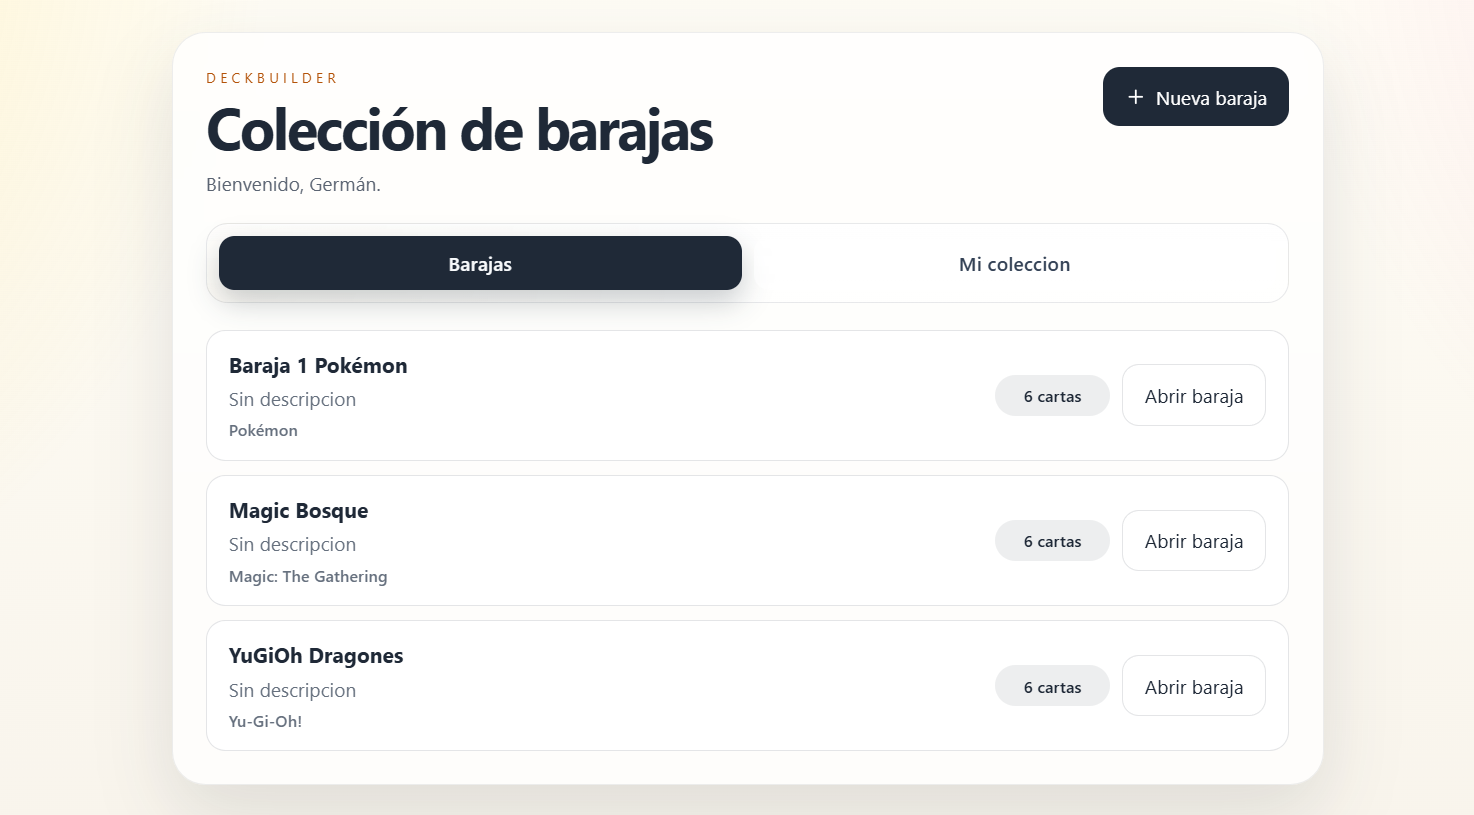
\includegraphics[width=0.9\textwidth]{figures/lista-barajas.png}
	\caption{Pantalla de colección de barajas}
	\label{fig:dev-frontend-lista-barajas}
\end{figure}

\begin{figure}[H]
	\centering
	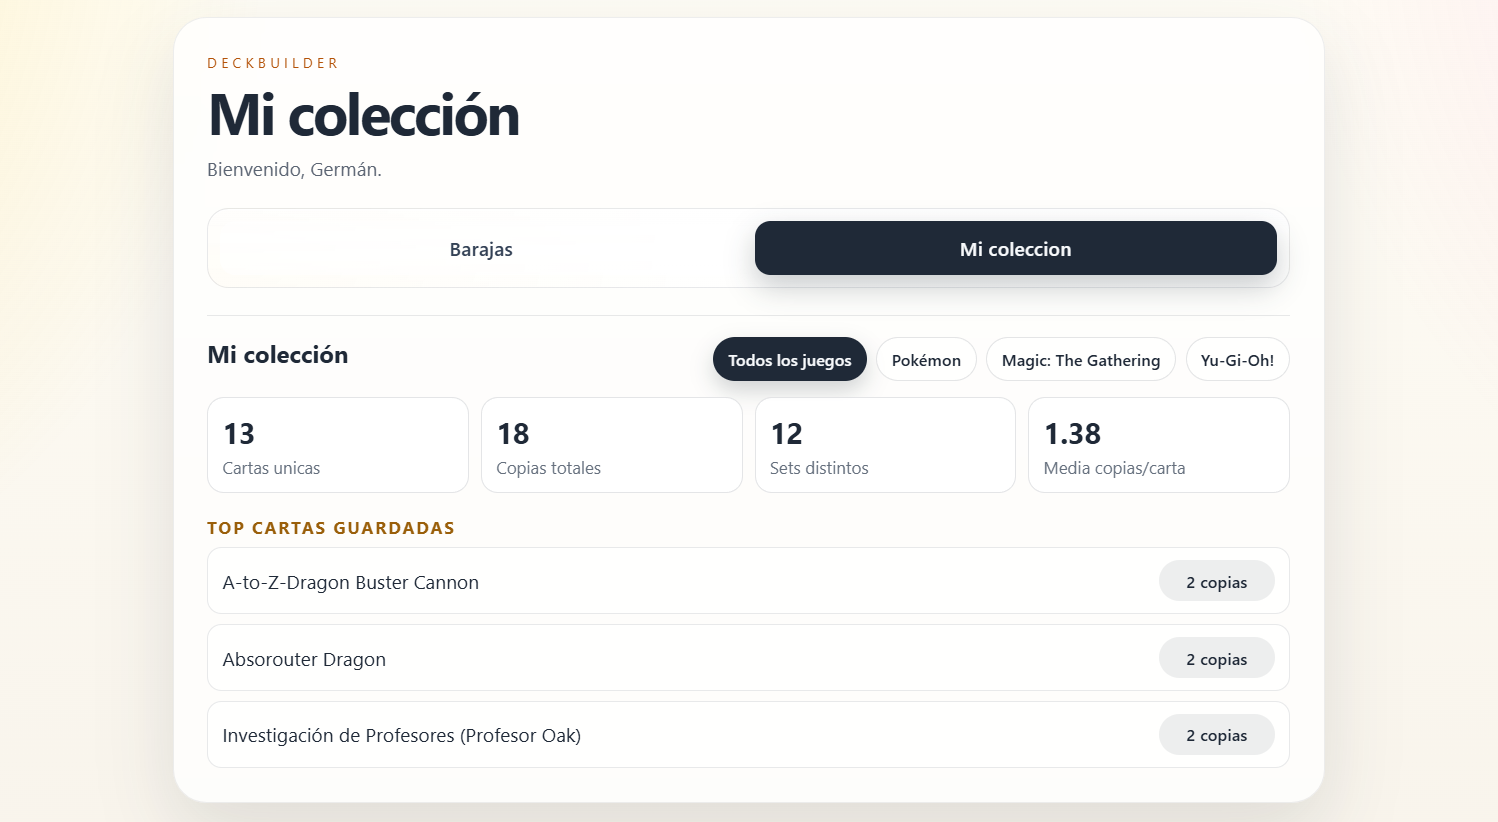
\includegraphics[width=0.9\textwidth]{figures/mi-coleccion.png}
	\caption{Pantalla de Mi colección}
	\label{fig:dev-frontend-mi-coleccion}
\end{figure}

\begin{figure}[H]
	\centering
	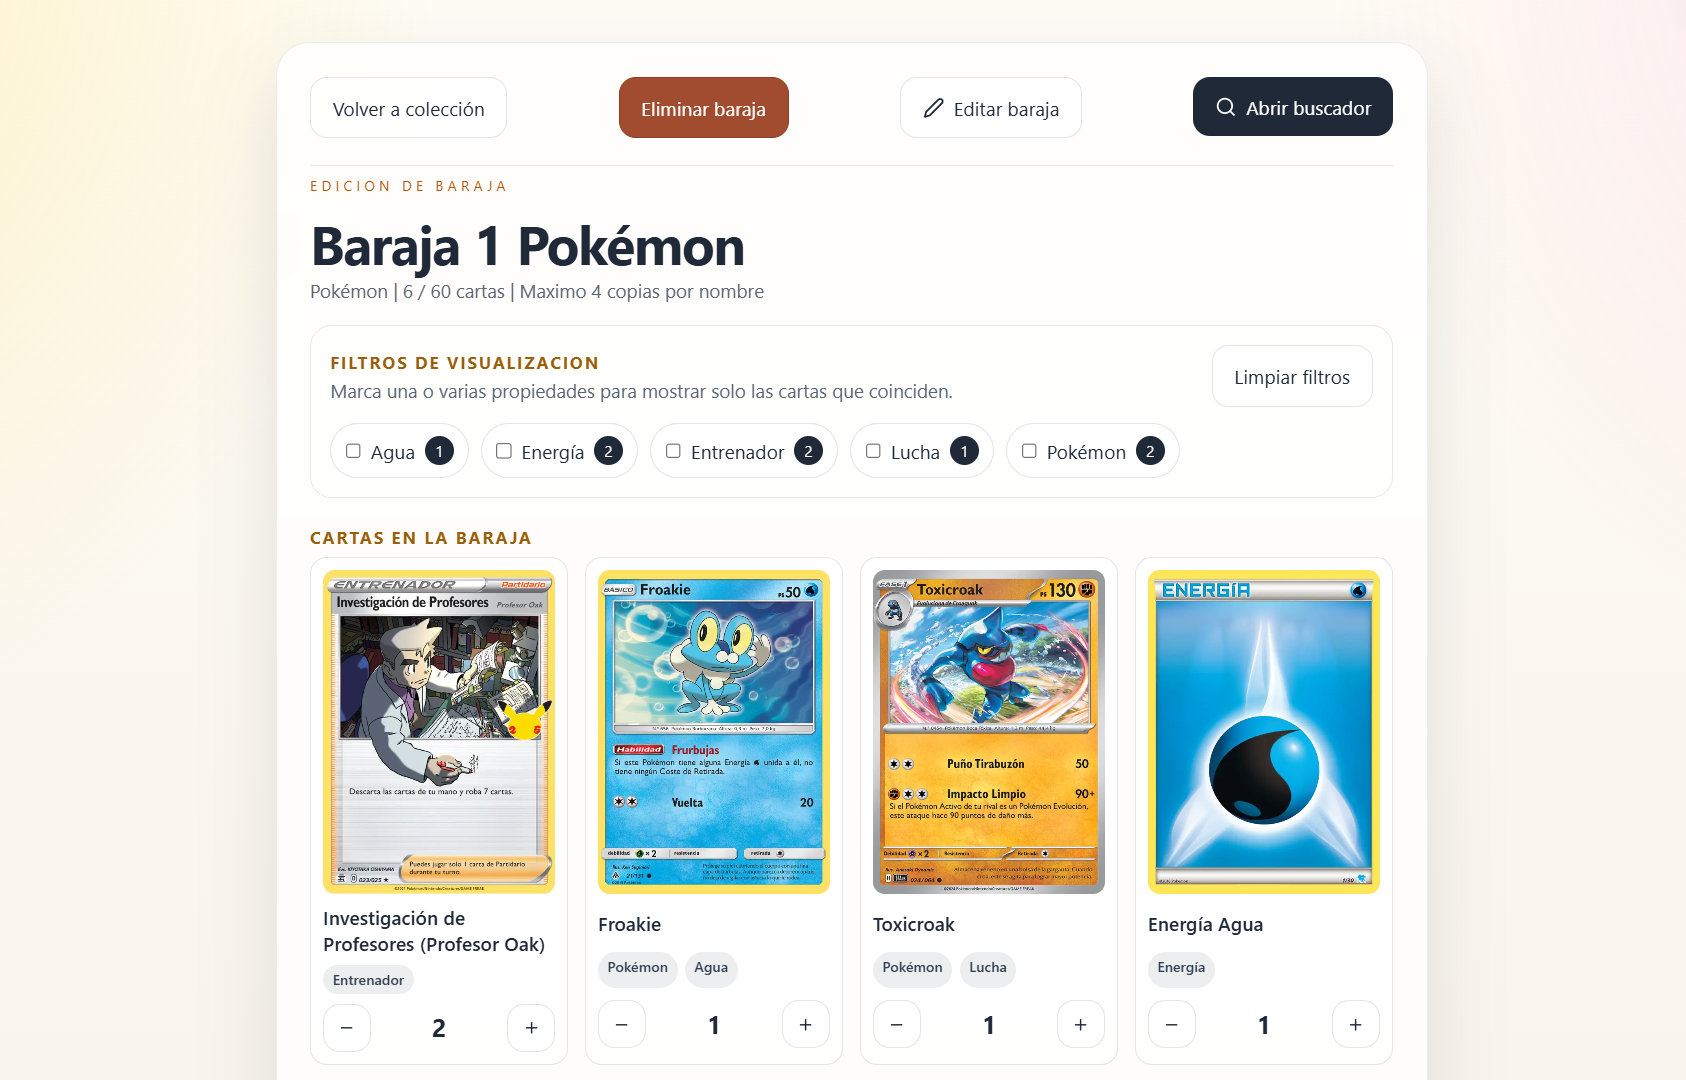
\includegraphics[width=0.9\textwidth]{figures/detalles-baraja.png}
	\caption{Pantalla de detalle y edición de baraja}
	\label{fig:dev-frontend-detalles-baraja}
\end{figure}

\begin{figure}[H]
	\centering
	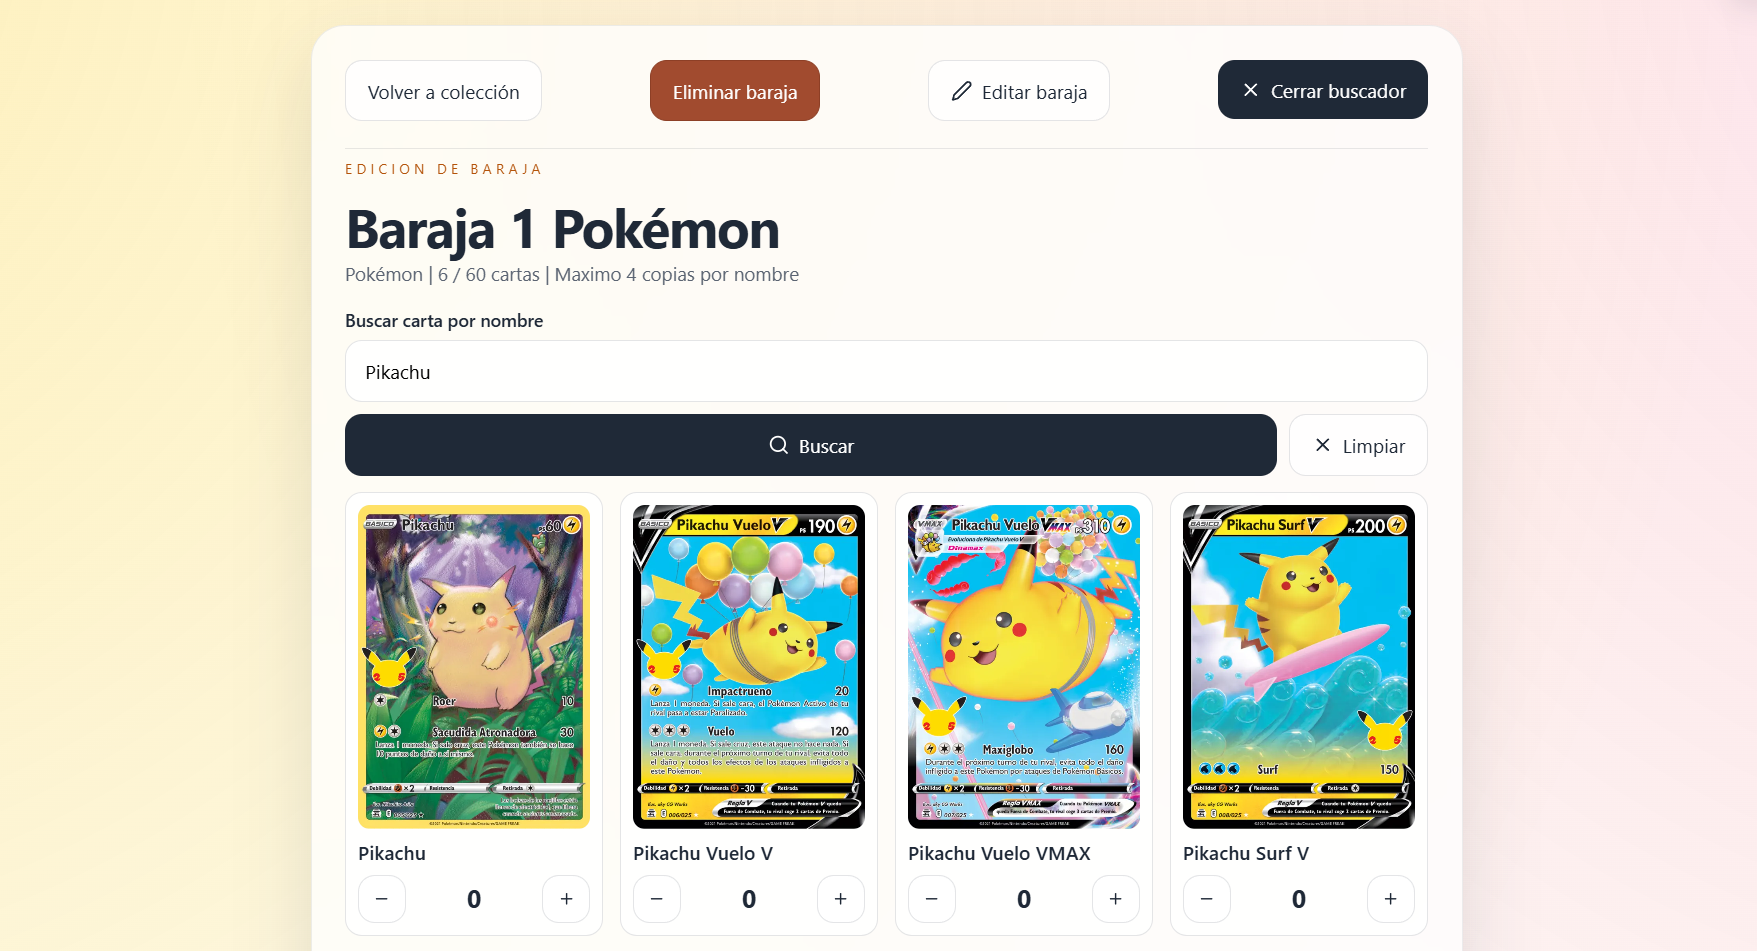
\includegraphics[width=0.9\textwidth]{figures/buscador.png}
	\caption{Pantalla de buscador de cartas}
	\label{fig:dev-frontend-buscador}
\end{figure}

\section{Capacidades multijuego y editor visual}

Una de las partes más relevantes de esta fase fue la transformación de la plataforma
en una solución multijuego auténtica. Se integra el tipo de juego (Pokémon, Magic o
Yu-Gi-Oh!) como un atributo estructural dentro de la base de datos de MongoDB,
permitiendo que el sistema se adapte dinámicamente según la elección del usuario al
crear una nueva baraja.

Gracias a esta base polimórfica, se desarrolló un endpoint de búsqueda unificado capaz
de consultar múltiples fuentes externas de manera homogénea. Esta integración permite
al usuario buscar cartas de diferentes franquicias bajo un mismo estándar visual,
simplificando la complejidad técnica de las diferentes estructuras de datos de origen.

Finalmente, se construyó el editor visual de barajas, la herramienta central de la
aplicación. En este componente, los usuarios pueden añadir o retirar cartas mediante
controles directos, mientras el sistema aplica automáticamente las reglas de validación
específicas de cada juego dentro de la lógica de actualización, garantizando que el
mazo resultante sea legal dentro de cada uno de los juegos.

El extracto \ref{cod:dev-multijuego-busqueda} resume la base de la implementación
multijuego: definir tipos de juego normalizados y seleccionar el proveedor de búsqueda
en función del valor recibido.

\begin{lstlisting}[language={[Sharp]C}, caption={DeckGameTypes simplificado y selección de proveedor (C\#)}, label={cod:dev-multijuego-busqueda}, captionpos=b]
public static class DeckGameTypes
{
    public const string Pokemon = "pokemon";
    public const string Magic = "magic";
    public const string Yugioh = "yugioh";
}

var cards = normalizedGameType switch
{
    DeckGameTypes.Pokemon => await SearchPokemonCardsAsync(httpClient, query, cancellationToken),
    DeckGameTypes.Magic => await SearchMagicCardsAsync(httpClient, query, cancellationToken),
    DeckGameTypes.Yugioh => await SearchYugiohCardsAsync(httpClient, query, cancellationToken),
    _ => []
};
\end{lstlisting}

\section{Resultados de la fase}

La Fase 2 concluyó exitosamente con un núcleo funcional operativo que integra
autenticación, vinculación de datos por usuario, un CRUD completo y un motor
multijuego. El sistema ha demostrado su funcionamiento al permitir la construcción de
mazos completos de forma muy clara e interactiva.

Desde el punto de vista arquitectónico, la solución queda preparada para crecer sin
necesidad de reestructurar la base de datos para cada nueva franquicia. Se ha logrado
una separación clara entre la interfaz, la lógica de negocio y la capa de persistencia,
dejando una base sólida para las próximas etapas.
